\documentclass[12pt]{article}%
\usepackage[T1]{fontenc}%
\usepackage[utf8]{inputenc}%
\usepackage{lmodern}%
\usepackage{textcomp}%
\usepackage{parskip}%
\usepackage{geometry}%
\geometry{margin=1.15cm}%
\usepackage{ragged2e}%
%
%------------------------------------------------------------------------------
%
% Automatically generated by make on 2021-06-12 
%
%------------------------------------------------------------------------------
%
\usepackage{graphicx}%
\usepackage{enumitem}%
\usepackage{url}%
\setcounter{secnumdepth}{0}%
\usepackage{titlesec}%
\titlespacing\section{0pt}{12pt}{12pt}%
\titlespacing\subsection{0pt}{12pt}{12pt}%
%
\begin{document}%
\pagestyle{empty}%
\normalsize%
\pagestyle{empty}%
\raggedright%
\begin{minipage}{0.45\textwidth}%
\centering%
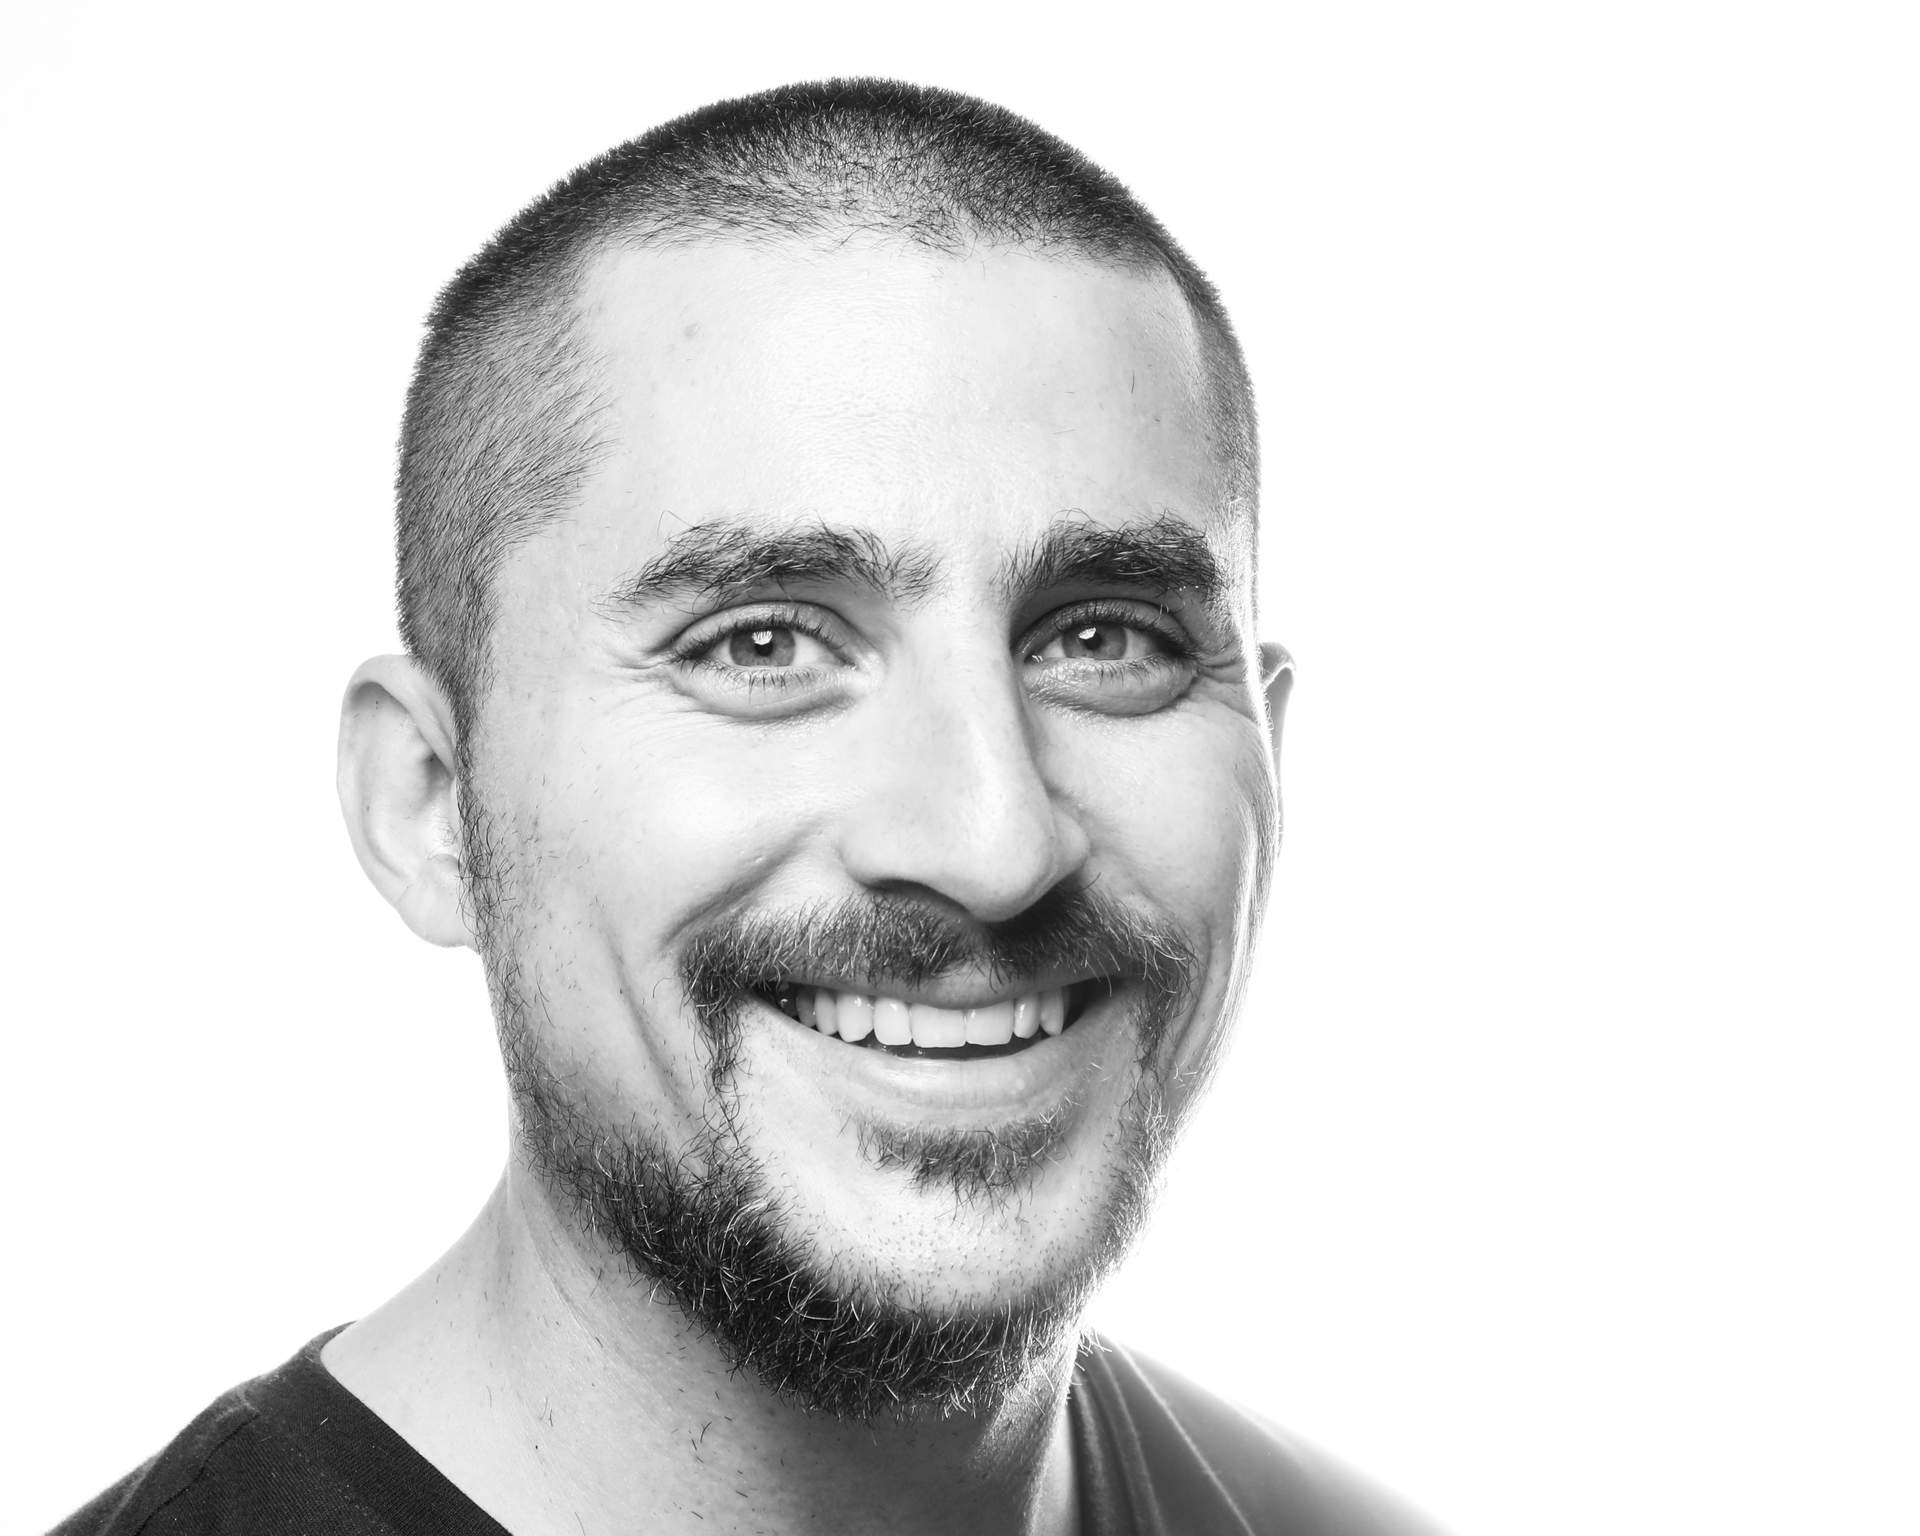
\includegraphics[width=200pt]{/Users/fd/Documents/cv/data/profil.jpg}%
\end{minipage}%
\begin{minipage}{0.6\textwidth}%
\section{Federico Nicolás Cámara Halac}%
\label{sec:FedericoNicolsCmaraHalac}%
\begin{itemize}[align=parleft,leftmargin=2.25cm,labelwidth=2cm]
\item[Phone]
+ 1 (614) 440{-}7529
\item[Email]
\url{camarahalac.1@osu.edu}
\item[Website]
\url{https://fdch.github.io}
\item[Address]
349C Sullivant Hall,\\1813 North High Street,\\Columbus, OH 43210
\item[Birth]
8th May 1988, Córdoba, Argentina
\end{itemize}

%
\end{minipage}%
\hfill%
\section{Education}%
\label{sec:Education}%
\hrule%
\subsection{PhD}%
\begin{itemize}[align=parleft,leftmargin=2.25cm,labelwidth=2cm]
\item[2019]
\textbf{Music Composition and Theory, New York University.}
Graduate School of Arts and Sciences. 
Dissertation title: ``Database Music: A History, Technology, and Aesthetics of the Database in Music Composition''. Advisor: Jaime Oliver La Rosa (NYU GSAS). Readers: Elizabeth Hoffman (NYU GSAS), Martin Daughtry (NYU GSAS), William Brent (American University), and Robert Rowe (NYU Steinhardt). 
New York, NY (USA). 
Sep  2013 {-} Jun  2019.
\end{itemize}%
\subsection{Licenciate}%
\begin{itemize}[align=parleft,leftmargin=2.25cm,labelwidth=2cm]
\item[2012]
\textbf{Music Composition, Universidad Nacional de Córdoba.}
Facultad de Artes. 
Thesis Title: ``A Form of Pleasure: Music as an Experience of Pleasure''. Advisor: José Halac. Readers: Eleazar Garzón, Sergio Poblete, Claudio Bazán, and Pablo de Giusto (Bachelor and Masters equivalence). 
Córdoba (Argentina). 
Mar  2006 {-} Jul  2012.
\end{itemize}

%
\section{Professional Appointments}%
\label{sec:ProfessionalAppointments}%
\hrule%
\subsection{Postdoctorate}%
\begin{itemize}[align=parleft,leftmargin=2.25cm,labelwidth=2cm]
\item[2021]
\textbf{Postdoctoral Scholar in Immersive Audio, The Ohio State University.}
Global Arts and Humanities Discovery Theme, School of Music, Advanced Computing Center for the Arts and Design. 
Columbus, OH (USA). 
2019{-}2021.
\end{itemize}%
\section{Research Interests}%
\label{sec:ResearchInterests}%
\begin{quote}
Computer Music. Spatial Audio. Immersive Sound. Machine Learning. Digital Signal Processing. Algorithmic Composition. Computer Vision. Networked Music Performance. Sonification. Database Music
\end{quote}

%
\pagebreak

%
\section{Publications}%
\label{sec:Publications}%
\hrule%
\subsection{Conference Proceedings}%
\begin{itemize}[align=parleft,leftmargin=2.25cm,labelwidth=2cm]
\item[2021 | Sep]
\textbf{Visual Cues as an Aid in the Auditory Stream Segregation of Music.}
International Conference on Music Perception and Cognition {-} European Society for the Cognitive Sciences of Music. 
Samantha Burgess, Federico Camara Halac, and Daniel Shanahan. 
28 September 2021.
\end{itemize}%
\begin{itemize}[align=parleft,leftmargin=2.25cm,labelwidth=2cm]
\item[August]
\textbf{`The Woods:' A Mixed Reality Two{-}Player Cooperative Game.}
SIGGRAPH. 
Scott Swearingen, Kyoung Swearingen, Federico Camara Halac, Sruthi Ammannagari, and Matt Hall. 
09 August 2021.
\end{itemize}%
\begin{itemize}[align=parleft,leftmargin=2.25cm,labelwidth=2cm]
\item[July]
\textbf{DreamSound: Deep Activation Layer Sonification.}
International Community for Auditory Displays. 
Federico Camara Halac and Matias Delgadino. 
25 July 2021.
\end{itemize}%
\begin{itemize}[align=parleft,leftmargin=2.25cm,labelwidth=2cm]
\item[February]
\textbf{Comparing Musical Performances of the `Goldberg Variations' Using Supervised Machine Learning Techniques.}
Future Directions of Music Cognition (Accepted but not presented). 
Arturo Barrios, Leo A. Glowacki, Lindsay Warrenburg, and Federico Camara Halac. 
12 February 2021.
\end{itemize}%
\begin{itemize}[align=parleft,leftmargin=2.25cm,labelwidth=2cm]
\item[2017 | Oct]
\textbf{A Spectral Experience: Self Convolution and Face Tracking.}
International Computer Music Conference (Accepted but not presented). 
11 October 2017.
\end{itemize}%
\subsection{Conference Poster}%
\begin{itemize}[align=parleft,leftmargin=2.25cm,labelwidth=2cm]
\item[2020]
\textbf{PathoSonic: Performing Sound In Virtual Reality Feature Space.}
New Interfaces for Musical Expression. 
Federico Camara Halac and Shadrick Addy. 
24 January 2020.
\end{itemize}%
\subsection{Conference Panel}%
\begin{itemize}[align=parleft,leftmargin=2.25cm,labelwidth=2cm]
\item[2020]
\textbf{{[}clone fd\_dacout{]}: real{-}time massively multichannel spatialization in Pure Data.}
Jornadas de Informática y Electrónica Musical {-} Espacios Sonoros. 
05 March 2020.
\end{itemize}%
\subsection{PhD Dissertation Defense}%
\begin{itemize}[align=parleft,leftmargin=2.25cm,labelwidth=2cm]
\item[2019]
\textbf{Database Music: A History, Technology, and Aesthetics of the Database in Music Composition.}
New York University. 
06 May 2019.
\end{itemize}%
\subsection{Guest Speaker}%
\begin{itemize}[align=parleft,leftmargin=2.25cm,labelwidth=2cm]
\item[2021 | Sep]
\textbf{A History of the Database in Computer Music.}
Festival Atemporáneas. 
13 September 2021.
\end{itemize}%
\begin{itemize}[align=parleft,leftmargin=2.25cm,labelwidth=2cm]
\item[2018 | Jun]
\textbf{Composing Database: Opening A Space For The Concept Of An Anarchic Unwork Of Art..}
Delian Academy for New Music. 
11 June 2018.
\end{itemize}%
\begin{itemize}[align=parleft,leftmargin=2.25cm,labelwidth=2cm]
\item[2016]
\textbf{Inopera: A Multimedia Work for Loadbang and Pure Data.}
Universidad Nacional de Córdoba. 
15 June 2016.
\end{itemize}%
\subsection{Other Publications}%
\begin{itemize}[align=parleft,leftmargin=2.25cm,labelwidth=2cm]
\item[2017]
\textbf{`For Young Years:' A Response To Elsa Justel's Marelle.}
Open Space Magazine {-} Issue 21 . 
10 August 2017.
\end{itemize}

%
\section{Awards and Honors}%
\label{sec:AwardsandHonors}%
\hrule%
\subsection{Fellowships}%
\begin{itemize}[align=parleft,leftmargin=2.25cm,labelwidth=2cm]
\item[2018 | Sep]
\textbf{Dean's Dissertation.}
Graduate School of Arts and Sciences (New York University). 
Berlin (Germany). 
\end{itemize}%
\begin{itemize}[align=parleft,leftmargin=2.25cm,labelwidth=2cm]
\item[January]
\textbf{Graduate Research Initiative.}
Provost (New York University). 
Florence (Italy). 
\end{itemize}%
\begin{itemize}[align=parleft,leftmargin=2.25cm,labelwidth=2cm]
\item[2017]
\textbf{Graduate Research Initiative.}
Provost (New York University). 
Paris (France). 
\end{itemize}%
\begin{itemize}[align=parleft,leftmargin=2.25cm,labelwidth=2cm]
\item[2013 | Sep]
\textbf{The Henry M. MacCracken Program.}
Graduate School of Arts and Sciences (New York University). 
New York City (USA). 
\end{itemize}%
\subsection{Prizes}%
\begin{itemize}[align=parleft,leftmargin=2.25cm,labelwidth=2cm]
\item[2015 | Jun]
\textbf{"Ciudad Invertida" (Selected Works).}
Elsa Justel (Fundación Destellos). 
Mar del Plata (Argentina). 
\end{itemize}%
\begin{itemize}[align=parleft,leftmargin=2.25cm,labelwidth=2cm]
\item[2014]
\textbf{"Venas" (Selected Works) .}
Elsa Justel (Fundación Destellos). 
Mar del Plata (Argentina). 
\end{itemize}%
\begin{itemize}[align=parleft,leftmargin=2.25cm,labelwidth=2cm]
\item[2011 | Jul]
\textbf{"Lagos" (Orchestral Premiere).}
Orquesta Sinfónica de la UNC {-} Músicas en Dirigible (Universidad Nacional de Córdoba). 
Córdoba (Argentina). 
\end{itemize}%
\subsection{Conference Funds}%
\begin{itemize}[align=parleft,leftmargin=2.25cm,labelwidth=2cm]
\item[2017]
\textbf{Student Senators Council.}
Graduate School of Arts and Sciences (New York University). 
Shanghai (China). 
\end{itemize}%
\subsection{Exchange Program}%
\begin{itemize}[align=parleft,leftmargin=2.25cm,labelwidth=2cm]
\item[2012]
\textbf{Programa Cuarto Centenario.}
Prosecretaría de Relaciones Internacionales (Universidad Nacional de Córdoba and Université de Montréal). 
Montréal (Canada). 
\end{itemize}

%
\section{Performances}%
\label{sec:Performances}%
\hrule%
\subsection{Solo}%
\begin{itemize}[align=parleft,leftmargin=2.25cm,labelwidth=2cm]
\item[2020 | Mar]
\textbf{Concierto de arte sonoro en Espacio B.}
Ricardo Barney \& Pedro Fraguela. 
Laptop. 
Espacio B {-} Madrid (Spain). 
04 March 2020.
\end{itemize}%
\begin{itemize}[align=parleft,leftmargin=2.25cm,labelwidth=2cm]
\item[2017 | Aug]
\textbf{Lorenz Variations.}
Cube Fest at Virginia Tech {-} Blacksburg, VA (USA). 
03 August 2017.
\end{itemize}%
\begin{itemize}[align=parleft,leftmargin=2.25cm,labelwidth=2cm]
\item[2016 | Oct]
\textbf{Opening Portals.}
Jessica Rosen. 
Bookentiometers. 
ShapeShifter Lab in Brooklyn {-} New York City, NY (USA). 
11 October 2016.
\end{itemize}%
\subsection{The Sonic Arts Ensemble at OSU}%
\begin{itemize}[align=parleft,leftmargin=2.25cm,labelwidth=2cm]
\item[2021 | Jun]
\textbf{8th Music and/as Process Conference: Networked Collaborative Processes 2021.}
Thornblower. 
Netty McNetface {-} Columbus, OH (USA). 
26 June 2021.
\end{itemize}%
\begin{itemize}[align=parleft,leftmargin=2.25cm,labelwidth=2cm]
\item[April]
\textbf{SEAMUS (TWELVE).}
Thornblower. 
CCRMA {-} Stanford, CA (USA). 
23 April 2021.
\end{itemize}%
\begin{itemize}[align=parleft,leftmargin=2.25cm,labelwidth=2cm]
\item[]
\textbf{Earth Day Art Model 2021.}
Thornblower. 
EDAM Festival {-} Indianapolis, IA (USA). 
22 April 2021.
\end{itemize}%
\begin{itemize}[align=parleft,leftmargin=2.25cm,labelwidth=2cm]
\item[]
\textbf{Sonic Arts Ensemble Live{-}Stream Performance.}
Thornblower. 
Netty McNetface {-} Columbus, OH (USA). 
06 April 2021.
\end{itemize}%
\begin{itemize}[align=parleft,leftmargin=2.25cm,labelwidth=2cm]
\item[2020 | Oct]
\textbf{Into The Multiverse.}
Thornblower. 
The Wexner Center for the Arts {-} Columbus, OH (USA). 
20 October 2020.
\end{itemize}%
\begin{itemize}[align=parleft,leftmargin=2.25cm,labelwidth=2cm]
\item[2019 | Sep]
\textbf{Sonic Arts Ensemble and Atelier Avant Austria present ``Virtuoso Chances''.}
Andreas Weixler, Se{-}Lien Chuang, Marc Ainger, Ann Stimmson, and the Sonic Arts Ensemble. 
Pure Data, joyosc, and a PS4 Controller. 
ACCAD Motion Lab {-} Columbus, OH (USA). 
23 September 2019.
\end{itemize}%
\subsection{Hijos de Distinta Madre}%
\begin{itemize}[align=parleft,leftmargin=2.25cm,labelwidth=2cm]
\item[2020 | May]
\textbf{Thanks to Federico Ragessi and Franco Pellini (Hijos de Distinta Madre),  Marmotas Dreams (Berenice Llorens and Constanza Pellicci) , and Jorge Castro (fisterni @ La Cúpula) for an amazing performance and night..}
Pure Data, joyosc, and a PS4 Controller. 
La Cúpula Galería de Arte {-} Córdoba (Argentina). 
09 May 2020.
\end{itemize}%
\begin{itemize}[align=parleft,leftmargin=2.25cm,labelwidth=2cm]
\item[2019 | Dec]
\textbf{HDDM + ffddcchh + Marmotas Dreams \& friends.}
Pure Data, joyosc, and a PS4 Controller. 
La Cúpula Galería de Arte {-} Córdoba (Argentina). 
21 December 2019.
\end{itemize}%
\begin{itemize}[align=parleft,leftmargin=2.25cm,labelwidth=2cm]
\item[]
\textbf{HDDM + ffddcchh.}
Pure Data, joyosc, and a PS4 Controller. 
Casa Mandarina {-} Córdoba (Argentina). 
19 December 2019.
\end{itemize}%
\begin{itemize}[align=parleft,leftmargin=2.25cm,labelwidth=2cm]
\item[]
\textbf{Mermetom + Fede Camara Halac.}
Mermetom (Gustavo Alcaraz \& Vero Guevara) and . 
Pure Data, joyosc, and a PS4 Controller. 
La Cúpula Galería de Arte {-} Córdoba (Argentina). 
08 December 2019.
\end{itemize}%
\subsection{Live Video and Electronics}%
\begin{itemize}[align=parleft,leftmargin=2.25cm,labelwidth=2cm]
\item[2017 | Jun]
\textbf{Electroacoustic Improvisations.}
Joan Bages i Rubi, Bernardo Barros, Kyle Motl, and Joan Marti Frasquier,. 
Midi controller and Laptop. 
NYU Waverly Labs r.220 {-} New York City, NY (USA). 
19 June 2017.
\end{itemize}%
\begin{itemize}[align=parleft,leftmargin=2.25cm,labelwidth=2cm]
\item[April]
\textbf{a.le.a.}
Talea Ensemble. 
Midi controller and networked Laptops. 
The Dimenna Center for Classical Music {-} New York City, NY (USA). 
07 April 2017.
\end{itemize}%
\begin{itemize}[align=parleft,leftmargin=2.25cm,labelwidth=2cm]
\item[2016 | Nov]
\textbf{Ciudad Invertida.}
RAGE THORMBONES. 
Laptop. 
ShapeShifter Lab {-} New York City, NY (USA). 
22 November 2016.
\end{itemize}%
\begin{itemize}[align=parleft,leftmargin=2.25cm,labelwidth=2cm]
\item[September]
\textbf{sk.}
TAK Ensemble. 
Laptop. 
Waverly Labs, r.220 {-} New York City, NY (USA). 
29 September 2016.
\end{itemize}%
\begin{itemize}[align=parleft,leftmargin=2.25cm,labelwidth=2cm]
\item[April]
\textbf{INOPERA.}
Loadbang Ensemble. 
Midi controller and Laptop. 
The Dimenna Center for Classical Music {-} New York City, NY (USA). 
20 April 2016.
\end{itemize}%
\begin{itemize}[align=parleft,leftmargin=2.25cm,labelwidth=2cm]
\item[2015 | Aug]
\textbf{Ciudad Invertida.}
Rocío Elizalde y Manuel Pastrana. 
Laptop. 
Bienal 3 en Composición e Investigación Musical {-} Córdoba (Argentina). 
20 August 2015.
\end{itemize}%
\begin{itemize}[align=parleft,leftmargin=2.25cm,labelwidth=2cm]
\item[February]
\textbf{Mise{-}En at German House.}
Samuel Marques. 
Pure Data live processing. 
German Consulate {-} New York City, NY (USA). 
06 February 2015.
\end{itemize}%
\begin{itemize}[align=parleft,leftmargin=2.25cm,labelwidth=2cm]
\item[2014 | Apr]
\textbf{Momenta Quartet Plays NYU Composers.}
Momenta Quartet. 
Laptop. 
NYU Silver Center r.220 {-} New York City, NY (USA). 
21 April 2014.
\end{itemize}%
\subsection{LEIM Ensemble}%
\begin{itemize}[align=parleft,leftmargin=2.25cm,labelwidth=2cm]
\item[2012 | Aug]
\textbf{Ciclo Experimentalia.}
Piano, Analog Synthesizer. 
Centro Cultural España Córdoba {-} Córdoba (Argentina). 
10 August 2012.
\end{itemize}%
\begin{itemize}[align=parleft,leftmargin=2.25cm,labelwidth=2cm]
\item[2011 | Nov]
\textbf{Summer Concert.}
Piano, Analog Synthesizer. 
Auditorio CePIA {-} Córdoba (Argentina). 
10 November 2011.
\end{itemize}%
\begin{itemize}[align=parleft,leftmargin=2.25cm,labelwidth=2cm]
\item[October]
\textbf{Teatro Acústico.}
Piano, Analog Synthesizer. 
Facultad de Artes, UNC {-} Córdoba (Argentina). 
02 October 2011.
\end{itemize}%
\begin{itemize}[align=parleft,leftmargin=2.25cm,labelwidth=2cm]
\item[September]
\textbf{Ciclo Contengo{-}Arte.}
Piano, Analog Synthesizer. 
Instituto Italiano de Cultura {-} Córdoba (Argentina). 
14 September 2011.
\end{itemize}%
\begin{itemize}[align=parleft,leftmargin=2.25cm,labelwidth=2cm]
\item[]
\textbf{Micro{-}Simposio de Análisis Musical.}
Piano, Analog Synthesizer. 
Facultad de Artes, UNC {-} Córdoba (Argentina). 
12 September 2011.
\end{itemize}%
\begin{itemize}[align=parleft,leftmargin=2.25cm,labelwidth=2cm]
\item[August]
\textbf{Winter Concert.}
Piano, Analog Synthesizer. 
Auditorio CePIA {-} Córdoba (Argentina). 
23 August 2011.
\end{itemize}%
\begin{itemize}[align=parleft,leftmargin=2.25cm,labelwidth=2cm]
\item[June]
\textbf{Ciclo Experimentalia.}
Piano, Analog Synthesizer. 
Centro Cultural España Córdoba {-} Córdoba (Argentina). 
20 June 2011.
\end{itemize}%
\begin{itemize}[align=parleft,leftmargin=2.25cm,labelwidth=2cm]
\item[May]
\textbf{TSONAMI.}
Piano, Analog Synthesizer. 
Centro Cultural Recoleta {-} Buenos Aires (Argentina). 
10 May 2011.
\end{itemize}%
\begin{itemize}[align=parleft,leftmargin=2.25cm,labelwidth=2cm]
\item[2010 | Dec]
\textbf{Nosocomio.}
Piano, Analog Synthesizer. 
Centro Cultural España Córdoba {-} Córdoba (Argentina). 
12 December 2010.
\end{itemize}%
\begin{itemize}[align=parleft,leftmargin=2.25cm,labelwidth=2cm]
\item[November]
\textbf{Summer Concert.}
Piano, Analog Synthesizer. 
Auditorio CePIA {-} Córdoba (Argentina). 
14 November 2010.
\end{itemize}%
\begin{itemize}[align=parleft,leftmargin=2.25cm,labelwidth=2cm]
\item[September]
\textbf{1st International Biennial of Music Composition and Education.}
Piano, Analog Synthesizer. 
Auditorio CePIA {-} Córdoba (Argentina). 
14 September 2010.
\end{itemize}%
\begin{itemize}[align=parleft,leftmargin=2.25cm,labelwidth=2cm]
\item[2009 | Jan]
\textbf{Performances and Workshops.}
Piano, Analog Synthesizer. 
LEIM Facultad de Artes {-} Córdoba (Argentina). 
01 January 2009.
\end{itemize}%
\subsection{Proyecto {[}Red{]} Ensemble}%
\begin{itemize}[align=parleft,leftmargin=2.25cm,labelwidth=2cm]
\item[2016 | Aug]
\textbf{Canon.}
Midi controller and Laptop. 
Centro Cultural Graciela Carena {-} New York City, NY (USA). 
06 August 2016.
\end{itemize}%
\begin{itemize}[align=parleft,leftmargin=2.25cm,labelwidth=2cm]
\item[2012 | Nov]
\textbf{Concert.}
Piano. 
Auditorio CePIA {-} Córdoba (Argentina). 
12 November 2012.
\end{itemize}%
\begin{itemize}[align=parleft,leftmargin=2.25cm,labelwidth=2cm]
\item[]
\textbf{Aniversario de la Facultad de Artes.}
Piano, Trumpet, Midi Controller. 
Auditorio CePIA {-} Córdoba (Argentina). 
01 November 2012.
\end{itemize}%
\begin{itemize}[align=parleft,leftmargin=2.25cm,labelwidth=2cm]
\item[September]
\textbf{John Cage Festival.}
Piano. 
Auditorio CePIA {-} Córdoba (Argentina). 
05 September 2012.
\end{itemize}%
\begin{itemize}[align=parleft,leftmargin=2.25cm,labelwidth=2cm]
\item[August]
\textbf{Concert at B2CIM.}
Piano, Trumpet, Midi Controller. 
Auditorio CePIA {-} Córdoba (Argentina). 
23 August 2012.
\end{itemize}%
\begin{itemize}[align=parleft,leftmargin=2.25cm,labelwidth=2cm]
\item[June]
\textbf{Concierto de Alquimistas.}
Piano. 
Aula Magna FCEFyN {-} Córdoba (Argentina). 
29 June 2012.
\end{itemize}%
\begin{itemize}[align=parleft,leftmargin=2.25cm,labelwidth=2cm]
\item[]
\textbf{Concierto Final de Tesis.}
Piano. 
Auditorio CePIA {-} Córdoba (Argentina). 
12 June 2012.
\end{itemize}%
\begin{itemize}[align=parleft,leftmargin=2.25cm,labelwidth=2cm]
\item[2011 | Oct]
\textbf{Congreso de Ciencias Humana.}
Electric Guitar. 
Escuela Monserrat {-} Córdoba (Argentina). 
20 October 2011.
\end{itemize}%
\begin{itemize}[align=parleft,leftmargin=2.25cm,labelwidth=2cm]
\item[September]
\textbf{Micro{-}Simposio de Análisis Musical.}
Piano. 
Aula Magna de la Facultad de Artes {-} Córdoba (Argentina). 
10 September 2011.
\end{itemize}%
\begin{itemize}[align=parleft,leftmargin=2.25cm,labelwidth=2cm]
\item[August]
\textbf{Arte Forum 2: Homage to Oscar Bazán.}
Piano. 
Auditorio CePIA {-} Córdoba (Argentina). 
18 August 2011.
\end{itemize}%
\begin{itemize}[align=parleft,leftmargin=2.25cm,labelwidth=2cm]
\item[July]
\textbf{Winter Concert.}
Electric Guitar, Piano. 
Auditorio CePIA {-} Córdoba (Argentina). 
10 July 2011.
\end{itemize}%
\begin{itemize}[align=parleft,leftmargin=2.25cm,labelwidth=2cm]
\item[2010 | Nov]
\textbf{Summer Concert.}
Conductor. 
Auditorio CePIA {-} Córdoba (Argentina). 
20 November 2010.
\end{itemize}%
\begin{itemize}[align=parleft,leftmargin=2.25cm,labelwidth=2cm]
\item[July]
\textbf{Ciclo La Máquina de Tiempo.}
Trumpet. 
Centro Cultural España Córdoba {-} Córdoba (Argentina). 
02 July 2010.
\end{itemize}%
\subsection{Other Roles}%
\begin{itemize}[align=parleft,leftmargin=2.25cm,labelwidth=2cm]
\item[2020 | Jan]
\textbf{CLIMATE GATHERING.}
Norah Zuniga Shaw. 
Max/MSP and Ipad. 
Movement Lab at Barnard College {-} New York City, NY (USA). 
15 January 2020.
\end{itemize}%
\begin{itemize}[align=parleft,leftmargin=2.25cm,labelwidth=2cm]
\item[2012 | Mar]
\textbf{Guest Pianist.}
LAMOI. 
Piano. 
Paseo del Buen Pastor {-} Córdoba (Argentina). 
10 March 2012.
\end{itemize}%
\begin{itemize}[align=parleft,leftmargin=2.25cm,labelwidth=2cm]
\item[2010 | Sep]
\textbf{Inserto Beat.}
Luisina Couto, Pablo Behm. 
Guitar. 
Cineclub Municipal Hugo del Carril {-} Córdoba (Argentina). 
18 September 2010.
\end{itemize}%
\begin{itemize}[align=parleft,leftmargin=2.25cm,labelwidth=2cm]
\item[March]
\textbf{Guest Pianist.}
Orquesta Sinfónica de Río Ceballos. 
Piano. 
Teatro Municipal {-} Río Ceballos, CBA (Argentina). 
12 March 2010.
\end{itemize}

%
\section{Teaching}%
\label{sec:Teaching}%
\hrule%
\subsection{Professor}%
\begin{itemize}[align=parleft,leftmargin=2.25cm,labelwidth=2cm]
\item[2021 | Mar]
\textbf{Computational Musicology 8824.}
The Ohio State University. 
School of Music. 
Columbus, OH (USA). 
Spring 2021.
\end{itemize}%
\begin{itemize}[align=parleft,leftmargin=2.25cm,labelwidth=2cm]
\item[September]
\textbf{Sonic Arts Ensemble.}
The Ohio State University. 
Advanced Computing Center for the Arts and Design. 
Columbus, OH (USA). 
Fall 2021.
\end{itemize}%
\begin{itemize}[align=parleft,leftmargin=2.25cm,labelwidth=2cm]
\item[2020 | Mar]
\textbf{Sonic Arts Ensemble.}
The Ohio State University. 
Advanced Computing Center for the Arts and Design. 
Columbus, OH (USA). 
Spring 2020.
\end{itemize}%
\begin{itemize}[align=parleft,leftmargin=2.25cm,labelwidth=2cm]
\item[2019 | Sep]
\textbf{Sonic Arts Ensemble.}
The Ohio State University. 
Advanced Computing Center for the Arts and Design. 
Columbus, OH (USA). 
Fall 2019.
\end{itemize}%
\begin{itemize}[align=parleft,leftmargin=2.25cm,labelwidth=2cm]
\item[2015]
\textbf{Harmony and Counterpoint I.}
New York University. 
Faculty of Arts and Science. 
New York, NY (USA). 
Fall 2015.
\end{itemize}%
\subsection{Course Assistant}%
\begin{itemize}[align=parleft,leftmargin=2.25cm,labelwidth=2cm]
\item[2016]
\textbf{Computer Music Theory and Techniques.}
New York University. 
Faculty of Arts and Science. 
New York, NY (USA). 
Fall 2016.
\end{itemize}%
\subsection{Teaching Assistant}%
\begin{itemize}[align=parleft,leftmargin=2.25cm,labelwidth=2cm]
\item[2015 | Mar]
\textbf{Harmony and Counterpoint II.}
New York University. 
Faculty of Arts and Science. 
New York, NY (USA). 
Spring 2015.
\end{itemize}%
\begin{itemize}[align=parleft,leftmargin=2.25cm,labelwidth=2cm]
\item[2014 | Sep]
\textbf{Harmony and Counterpoint I.}
New York University. 
Faculty of Arts and Science. 
New York, NY (USA). 
Fall 2014.
\end{itemize}%
\begin{itemize}[align=parleft,leftmargin=2.25cm,labelwidth=2cm]
\item[2010 | Jan]
\textbf{Composición Musical I.}
Universidad Nacional de Córdoba. 
Facultad de Artes. 
Córdoba, CBA (ARG). 
\end{itemize}%
\begin{itemize}[align=parleft,leftmargin=2.25cm,labelwidth=2cm]
\item[2009]
\textbf{Composición Musical I.}
Universidad Nacional de Córdoba. 
Facultad de Artes. 
Córdoba, CBA (ARG). 
\end{itemize}%
\begin{itemize}[align=parleft,leftmargin=2.25cm,labelwidth=2cm]
\item[2008]
\textbf{Audioperceptiva I.}
Universidad Nacional de Córdoba. 
Escuela de Artes {-} FFyH. 
Córdoba, CBA (ARG). 
\end{itemize}%
\begin{itemize}[align=parleft,leftmargin=2.25cm,labelwidth=2cm]
\item[2007]
\textbf{Audioperceptiva I.}
Universidad Nacional de Córdoba. 
Escuela de Artes {-} FFyH. 
Córdoba, CBA (ARG). 
\end{itemize}

%
\section{Artistic Collaborations}%
\label{sec:ArtisticCollaborations}%
\hrule%
\subsection{Networked Music Performance}%
\begin{itemize}[align=parleft,leftmargin=2.25cm,labelwidth=2cm]
\item[2021 | Jan]
\textbf{1002: A Networked Music Performance with CollidePd}
(ongoing). 
International Computer Music Conference. 
Federico Ragessi. 
Córdoba (Argentina). 
\end{itemize}%
\begin{itemize}[align=parleft,leftmargin=2.25cm,labelwidth=2cm]
\item[2020 | Mar]
\textbf{The Sonic Arts Ensemble at OSU}
(ongoing). 
Advanced Computing Center for the Arts and Design. 
Marc Ainger and Ann Stimson. 
Columbus, OH (USA). 
\end{itemize}%
\subsection{Installations}%
\begin{itemize}[align=parleft,leftmargin=2.25cm,labelwidth=2cm]
\item[2019 | Sep]
\textbf{The Woods}
(ongoing). 
Advanced Computing Center for the Arts and Design. 
Kyoung Swearingen, Scott Swearingen, Marc Ainger, Sruthi Ammanngari, and Matt Hall. 
Columbus, OH (USA). 
\end{itemize}%
\begin{itemize}[align=parleft,leftmargin=2.25cm,labelwidth=2cm]
\item[2017 | Oct]
\textbf{Hearing the Self: A Spectral Experience.}
Xuhui Art Museum. 
Matias Delgadino and Lucia Simonelli. 
Shanghai (China). 
\end{itemize}%
\subsection{Theatre}%
\begin{itemize}[align=parleft,leftmargin=2.25cm,labelwidth=2cm]
\item[2013 | Oct]
\textbf{Poroto.}
Pabellón Azul {-} UNC . 
Celeste Lozada and Valentina Echeverría. 
Córdoba (Argentina). 
\end{itemize}%
\begin{itemize}[align=parleft,leftmargin=2.25cm,labelwidth=2cm]
\item[2012 | Sep]
\textbf{Itinerante: un Viaje a Través de Los Sentidos.}
Sindicato de Vendedores de Diarios y Revistas. 
Agustina Muñoz. 
Córdoba (Argentina). 
\end{itemize}%
\begin{itemize}[align=parleft,leftmargin=2.25cm,labelwidth=2cm]
\item[2011 | May]
\textbf{Tesis de Licenciatura de Teatro.}
Plazoleta del Fundador. 
Luisina Couto. 
Córdoba (Argentina). 
\end{itemize}%
\begin{itemize}[align=parleft,leftmargin=2.25cm,labelwidth=2cm]
\item[2010 | Apr]
\textbf{Inserto Beat.}
Cineclub Municipal Hugo del Carril. 
Luisina Couto. 
Córdoba (Argentina). 
\end{itemize}%
\subsection{Other Collaborations}%
\begin{itemize}[align=parleft,leftmargin=2.25cm,labelwidth=2cm]
\item[2013 | Feb]
\textbf{Los Chicos de Abril (Opera).}
Teatro Municipal de Río Cuarto. 
Luis Perez, Pablo Behm, and Franco Pellini. 
Río Cuarto , CBA (Argentina). 
\end{itemize}%
\begin{itemize}[align=parleft,leftmargin=2.25cm,labelwidth=2cm]
\item[2011 | Aug]
\textbf{Al Cielo o al Infierno (Film).}
Cines Gran Rex. 
Lauro Racosky. 
Córdoba (Argentina). 
\end{itemize}%
\begin{itemize}[align=parleft,leftmargin=2.25cm,labelwidth=2cm]
\item[2010 | May]
\textbf{Alicia en el País de las Maravillas (Dance).}
Teatro del Libertador San Martín. 
José Halac. 
Córdoba (Argentina). 
\end{itemize}

%
\section{Service}%
\label{sec:Service}%
\hrule%
\subsection{Disciplinary Service}%
\begin{itemize}[align=parleft,leftmargin=2.25cm,labelwidth=2cm]
\item[2020 | Jan]
\textbf{New Interfaces for Musical Expression}
(ongoing). 
Reviewer. 
Paper and Installation submissions. 
New York City (USA). 
\end{itemize}%
\begin{itemize}[align=parleft,leftmargin=2.25cm,labelwidth=2cm]
\item[2019]
\textbf{Festival Atemporáneas.}
Reviewer. 
Installation, Audiovisual, and Sound Art submissions. 
Buenos Aires (Argentina). 
2019{-}2020.
\end{itemize}%
\begin{itemize}[align=parleft,leftmargin=2.25cm,labelwidth=2cm]
\item[2018]
\textbf{New York City Electroacoustic Music Festival}
(ongoing). 
Reviewer. 
Music submissions. 
New York City (USA). 
\end{itemize}%
\begin{itemize}[align=parleft,leftmargin=2.25cm,labelwidth=2cm]
\item[]
\textbf{International Computer Music Conference}
(ongoing). 
Reviewer. 
Installations and Music Submissions. 
New York City (USA). 
\end{itemize}%
\begin{itemize}[align=parleft,leftmargin=2.25cm,labelwidth=2cm]
\item[2016]
\textbf{PdCon16\textasciitilde{}.}
Organizer. 
Website and Conference Program. 
New York City (USA). 
\end{itemize}%
\begin{itemize}[align=parleft,leftmargin=2.25cm,labelwidth=2cm]
\item[2010]
\textbf{Bienal Composición Córdoba.}
Organizer. 
Website and Conference Program. 
Córdoba (Argentina). 
2010{-}2015.
\end{itemize}%
\subsection{University Service}%
\begin{itemize}[align=parleft,leftmargin=2.25cm,labelwidth=2cm]
\item[2013 | Jan]
\textbf{Waverly Project.}
Founding Member. 
Website and Program. 
New York City (USA). 
2013{-}2017.
\end{itemize}%
\begin{itemize}[align=parleft,leftmargin=2.25cm,labelwidth=2cm]
\item[2010]
\textbf{Proyecto {[}Red{]} Ensamble.}
Founding Member. 
Website and Program. 
Córdoba (Argentina). 
2010{-}2015.
\end{itemize}

%
\section{Other Skills}%
\label{sec:OtherSkills}%
\hrule%
\begin{itemize}[align=parleft,leftmargin=2.25cm,labelwidth=2cm]
\item[Languages]
\textbf{Spanish}
 (Native) 
\textbf{English}
 (Advanced) 
\textbf{French}
 (Intermediate) 
\textbf{German}
 ( Beginner, A2 Level. Currently Studying.) 
\item[Code]
\textbf{Pure Data}
 (Expert) 
\textbf{Python}
 (Advanced: Numpy, Scipy, tensorflow, librosa) 
\textbf{JavaScript}
 (Advanced: Web Audio API, Node.js) 
\textbf{C}
 (Pure Data Externals) 
\textbf{C++}
 (GEM and Max MSP Externals) 
\textbf{Bash}
 (Server{-}side scripting) 
\textbf{HTML}
 (Web Publishing with CSS) 
\textbf{Latex}
 (Text Publishing) 
\textbf{Git}
 (Version management, software release) 
\item[Software]
\textbf{Max/MSP.}
\textbf{Csound.}
\textbf{Jacktrip.}
\textbf{Audacity.}
\textbf{REAPER.}
\textbf{Ableton Live.}
\textbf{Adobe Creative Suite.}
\end{itemize}

%
\end{document}